\documentclass{article}

\usepackage{a4wide}
\usepackage[utf8]{inputenc}
\usepackage[T1]{fontenc}
\usepackage[french]{babel}
\usepackage[babel=true]{csquotes} % guillemets français
\usepackage{graphicx}
\graphicspath{{Images/}}
\usepackage{color}
\usepackage{hyperref}
\hypersetup{colorlinks,linkcolor=,urlcolor=blue}

\usepackage{amsmath}
\usepackage{amssymb}


\title{Balles en Mouvement}
\author{Brahim Sirine, L3 informatique}
\date{\today}

\begin{document}

\maketitle % pour écrire le titre


%% Le résumé:
\begin{abstract}
Cette petite application a pour but est pour bien comprendre le langage java, la programmation orientée objet et le fonctionnement général des threads \cite{thread} et de l'ordonnanceur car en général il est impossible de développer une application robuste n'importe comment en java.
\end{abstract}

\section{Introduction}
\label{section:hello} % pour faire référence à la section ailleurs (\ref{...} voir plus bas)
j'ai choisi l'exercice des balles en mouvement comme application à réaliser est pour but de bien comprendre la fonctionnement des threads, leurs synchronization et leurs ordonnancement.et je trouve que cet exercice est un exemple concret et efficace pour avancer a apprendre le langage java .Pour ce faire je vais détailler tout les étapes de mon propre raisonnement.
 

\section{\'Etude préliminaire}
Cette technique consiste à préparer une interface graphique de l'application qui permette d'ajuster les besoins et de les concevoir de manière précise. En effet, cette interface graphique donne une vision claire de l'application avant sa réalisation et qui permet de de bien entamer le projet.

\begin{center}
  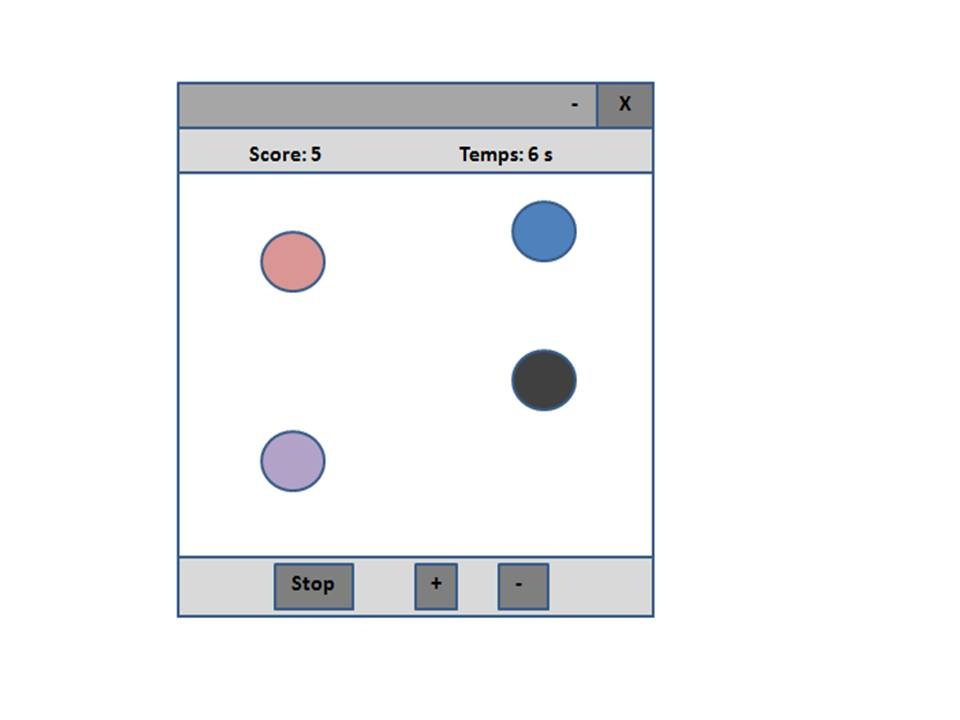
\includegraphics[scale=0.5]{yy.JPG}
\end{center}
Cette figure exprime les détails de l'interface graphique et qui permet à l'utilisateur d'interagir avec les Balles dedans. Cette maquette contient des labels et des boutons. Dans la partie supérieure à gauche il y a un label qui indique le score affiché en permanence et incrémenté a chaque collision et à la partie supérieure à droite il y a un label horloge qui affiche le temps écoulé pendant que les balles sont en mouvement: cette horloge stoppe son décompte lorsque les balles sont arrêtées et reprendre son décompte lorsque les balles sont à nouveau en mouvement. Et au milieu de la fenêtre il existe les balles en mouvement et qui ne peuvent pas sortir de la fenêtre et ricochent contre les bords. Mais lorsque une collision se produit, les balles impliquées sont supprimées.
Cette maquette présente aussi des boutons dans la partie inférieure de la fenêtre, le premier bouton permet de "démarrer/arrêter" le mouvement de toutes les balles. Lorsque les balles sont en mouvement, ce bouton a pour étiquette “stop” et lorsque les balles sont à l'arrêt il a pour étiquette “start”. Un autre bouton “+” permet d’ajouter une nouvelle balle de couleur aléatoire. Lorsqu’un seuil fixé au préalable est atteint, plus aucune balle ne peut être ajoutée. et l'autre bouton “-” permet de supprimer une balle.
% \cite{...} permet de faire référence à des éléments de la
% bibliographie.

\section{Architecture Générale}
Tout d'abord j'ai commencé la réalisation de mon application par développer mon interface graphique comme montre la figure ci dessous.Mon interface est presque la même que celle réaliser dans la partie étude préliminaire .Et pour l'implémentation de mon application, j'ai utilisé l'eclipse comme logiciel.
\begin{center}
  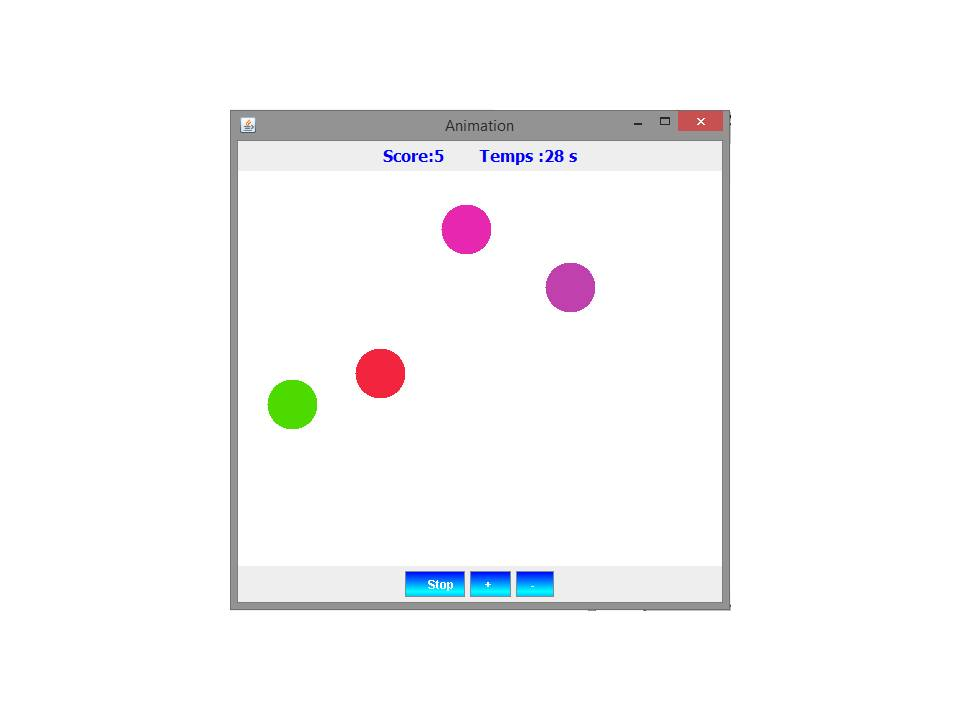
\includegraphics[scale=0.5]{Diapo1.JPG}
\end{center}
Maintenat, dans cette section je vais présenter l'implémentation des différentes parties de mon application.Tout d'abord je vais montrer l'implémentation de l'interface graphique, les labels, les boutons etc...:
\begin{center}
  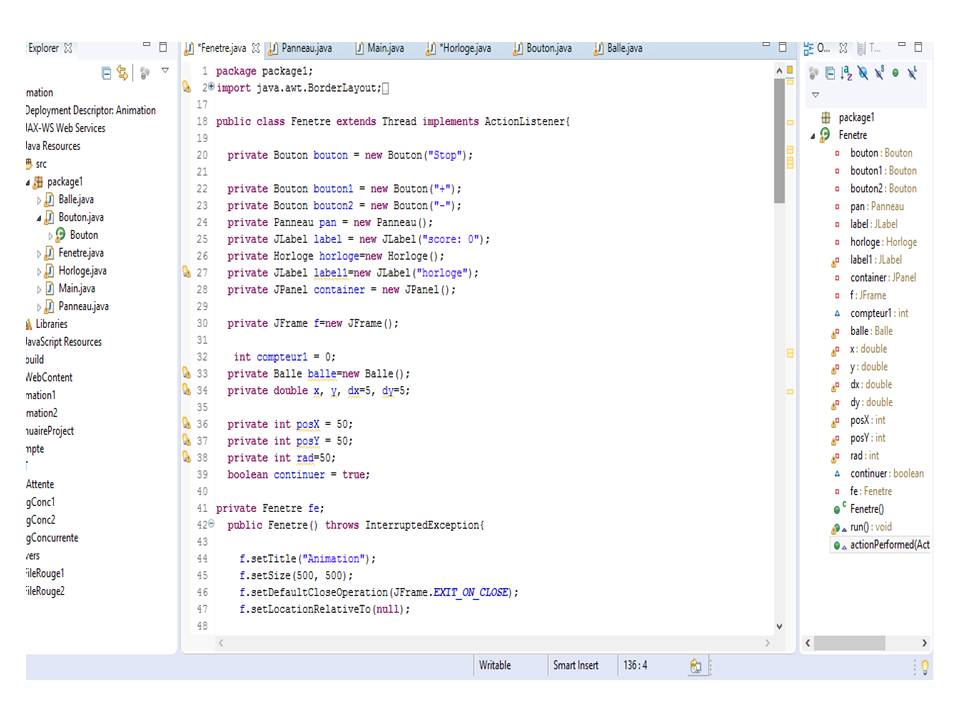
\includegraphics[scale=0.5]{kk.JPG}
\end{center}
\begin{center}
  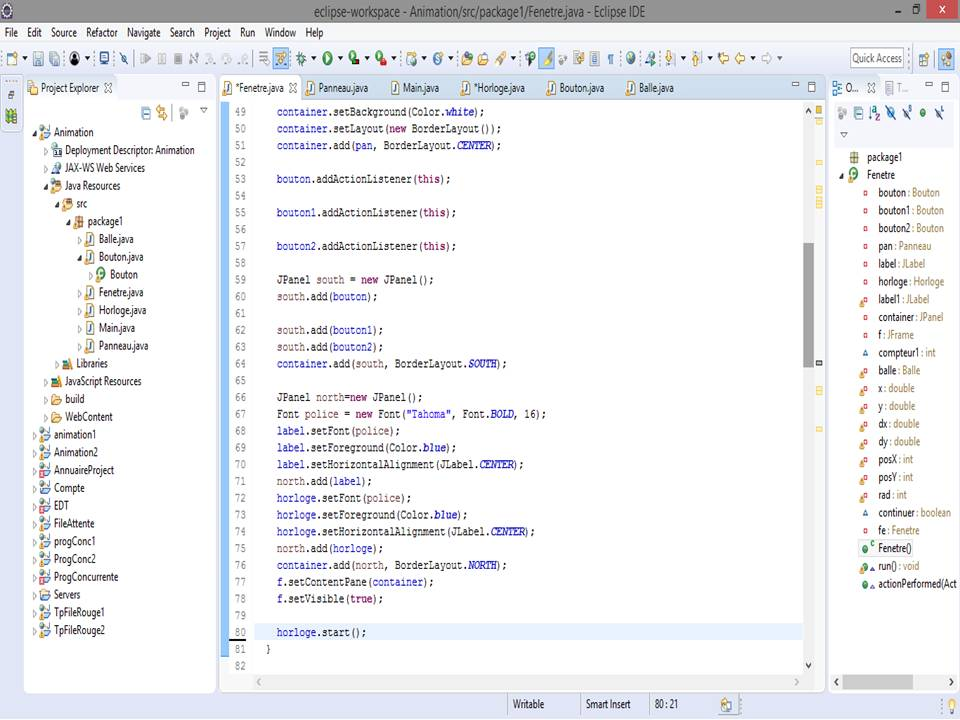
\includegraphics[scale=0.5]{gg.JPG}
\end{center}

Cette classe présente la fenêtre de mon interface qui hérite de la classe thread et qui implémente de l'interface ActionListener .
\\
\\
Dans cette classe, j'ai utilisé la méthode run() ci-dessous qui contient en générale le code des traitements qui seront exécutés dans le thread. Et dans cette méthode j'ai utilisé le mot Synchronized\cite{synchronized} pour assurer la sureté et la vivacité de mon programme. Par exemple ici dans mon programme ,les balles doivent être exécutés séquentiellement.

\begin{verbatim}
 public void run() {
 
	while(continuer) {
			try
			  {
			    continuer=true;
			   	pan.deplacer();	
				pan.Collision();			
		    	f.setContentPane(container);
			    fe.sleep(10);
				pan.repaint();
				compteur1=pan.compteur;
				label.setText("Score:" + this.compteur1+"      ");
			  }
			catch (InterruptedException exc) {}
}
		
			try
				 {
			      sleep(200); 
				 synchronized(this)
				      {	   
					while (!continuer) wait();
				     
				      }
				    continuer=true;
				  }
				catch (InterruptedException exc) {}
		
		      }
\end{verbatim}
\begin{center}
  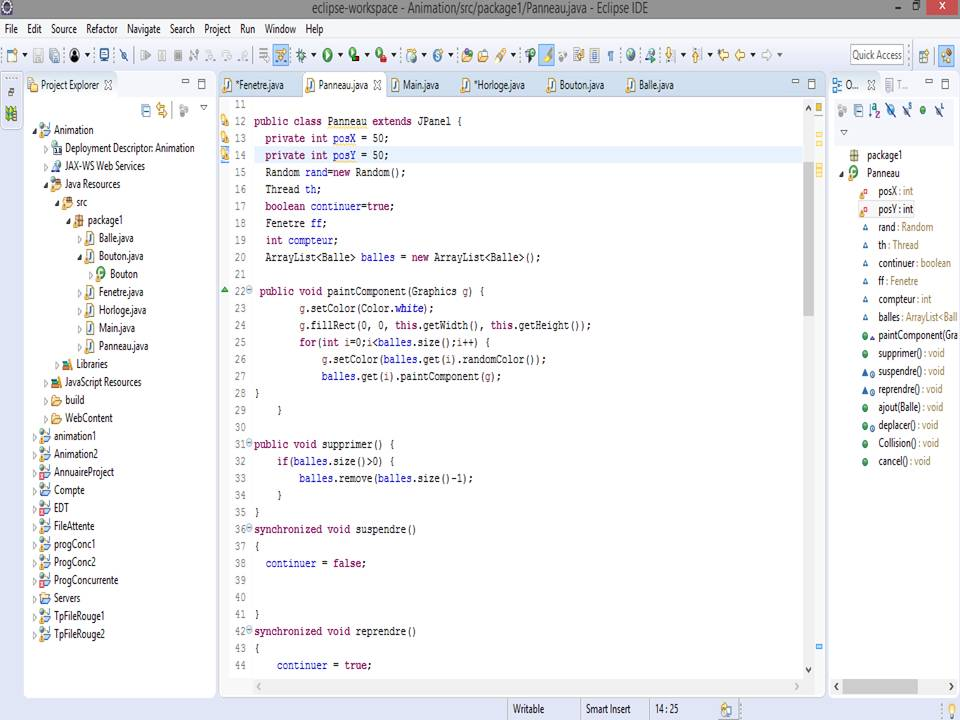
\includegraphics[scale=0.5]{ss.JPG}
\end{center}

La figure ci-dessus montre l'implémentation de mon panneau qui hérite de JPanel .Cette Classe permet d'organiser les différents éléments dans la fenêtre: les labels et les boutons .Et Dans cette classe j'ai utilisé une méthode "Ajout" qui a le rôle d'ajouter les balles dans la fenêtre. Dans cette méthode,j'ai utilisé Une Liste des balles afin de gérer facilement l'ensemble des balles.Et voila mon bout de code que j'ai implémenté.

\begin{verbatim}
  public void ajout(Balle balle) {
	if(balles.size()<100) {
		int maxX=this.getWidth();
		int maxY=this.getHeight();
	if(rand.nextFloat()>0.5) {
		balle.setDirectX(1);
	}else {
		balle.setDirectX(-1);
	}
	if(rand.nextFloat()>0.5) {
		balle.setDirectY(1);
	}else {
		balle.setDirectY(-1);
	}
	balle.posX=balle.dx+(int)(rand.nextFloat()*(((maxX-balle.dx)+1)));
	balle.posY=balle.dx+(int)(rand.nextFloat()*(((maxY-balle.dx)+1)));
	balles.add(balle);}
	}
\end{verbatim}

J'ai utilisé aussi la méthode deplacer() qui permet de rebondir les balles dans la fenêtre.Et dans cette méthode j'ai créer une boucle qui va parcourir tous les éléments de la Liste pour les déplacer. Et voila mon bout de code:

\begin{verbatim}
 public synchronized void deplacer()throws InterruptedException{
		 for(int i=0;i<balles.size();i++) {
			  balles.get(i).setPosX(balles.get(i).posX+balles.get(i).getDirectX());
			  balles.get(i).setPosY(balles.get(i).posY+balles.get(i).getDirectY());
			  balles.get(i).repaint();
			  
			  if(balles.get(i).getPosX()>this.getWidth()-balles.get(i).dx) balles.get(i).setDirectX(-1);
			  if(balles.get(i).getPosY()>this.getHeight()-balles.get(i).dx) balles.get(i).setDirectY(-1);
			  
			  if(balles.get(i).getPosX()<=0) balles.get(i).setDirectX(1);
			  if(balles.get(i).getPosY()<=0) balles.get(i).setDirectY(1);
			 }
 }
\end{verbatim}

 la classe Horloge ci dessous est une classe qui hérite de la classe JLabel son rôle principale est d'afficher le temps écoulé pendant que les balles sont en mouvement.Cette horloge permet de stopper son décompte lorsque les balles sont arrêtées grâce à la méthode Stop() et aussi permet de reprendre  son décompte lorsque les balles sont à nouveau en mouvement grâce à la méthode Start() .
\begin{center}
  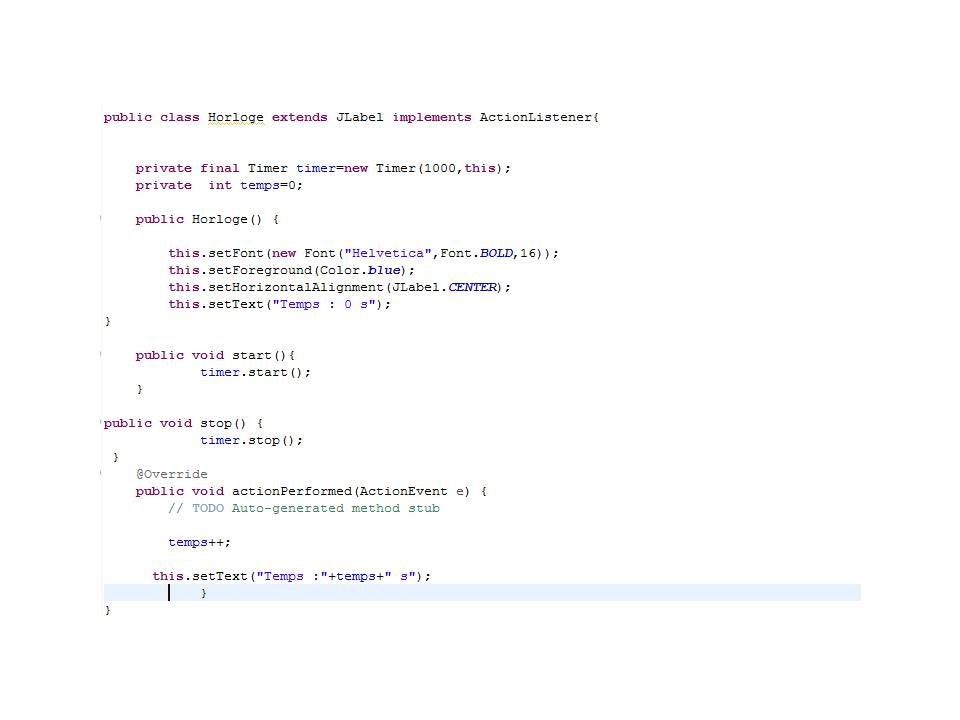
\includegraphics[scale=0.5]{hor.JPG}
\end{center}
Aussi,J'ai créer une classe Balle avec les deux attributs posX et posY qui sont les positions de la balle à l'écran, et directX et directY qui sont les directions du mouvement de la balle, et dans cette classe j'ai implémenté une méthode paintComponent(Graphics g) qui affiche la balle à l'écran en fonction de la posX et posY et la taille qui est dx.j'ai implémenté aussi les getters et les setters des variables initialisées pour donner l'accées à ces variables depuis l'extérieur de la classe.
\\
\\
\\

Et enfin, afin d'exécuter tout mon programme, j'ai implémenter la méthode main ci dessous: \cite{Openclassr}
\begin{verbatim}
public class Main {
public static void main(String args[]) throws InterruptedException {
	Fenetre fen = new Fenetre();
	fen.start();	
}
}
\end{verbatim}

\section{La Conclusion}

% \ref{...} permet de faire référence à un élément défini
% ailleurs dans le document (voir \label{...} plus haut).
Le présent travail consiste à la réalisation d'une petite application des balles en mouvement.
j'ai présenté dans cet rapport toutes les étapes que j'ai suivi pour la réalisation de cette application tout en spécifiant les méthodes que j'ai implémenté  en présentant des quelques imprimes d'écrans et quelques bouts de code de l'application.  

\section{Bibliographie}



%%% La bibliographie:
\bibliographystyle{plain}
\bibliography{bib2}

\end{document}
